%--------------------------------------------------------------------------
\chapter{Testing laryngeal complexity in SLZ} \label{ch:testing_lc}
%--------------------------------------------------------------------------

%--------------------------------------------------------------------------
\section{Introduction}\label{sec:introduction_of_lc}
%--------------------------------------------------------------------------

This chapter investigates the role that laryngeal complexity plays in Santiago Laxopa Zapotec. Laryngeal complexity is used to describe the contrastive use of tone and phonation in many languages, especially in the Oto-Manguean languages \citep{blankenshipTimeCourseBreathiness1997,blankenshipTimingNonmodalPhonation2002,silvermanLaryngealComplexityOtomanguean1997,silvermanPhasingRecoverability1997}. As mentioned in Chapter~\ref{ch:SLZ}, SLZ is a laryngeally complex language, because of its contrastive use of both tone and phonation. This means that SLZ can be used to test the predictions of laryngeal complexity, with respect to the phasing and recoverability of tone and phonation.

The goal of this chapter is to show that laryngeal complexity is present in SLZ as evidenced by the phasing of nonmodal phonation in several acoustic measures. This is done by looking at the acoustic properties of SLZ phonation using a combination of Strength of Excitation (SoE), Harmonic-to-Noise Ratio (HNR) < 1500 Hz and \textit{f}0 perturbations. It will be shown that there is a clear phasing between modal and nonmodal phonation in vowels that are described as breathy, checked, and rearticulated. 

These measures were selected based on the results of the MDS analysis in Chapter~\ref{ch:acousticlandscape} and the Random Forest analysis in Chapter~\ref{ch:revealing_trees}. Both MDS and Random Forest analyses showed that SoE and HNR < 1500 Hz were the most important measures to distinguish between the different types of phonation. SoE has previously been used to show that there is a clear phasing between modal and rearticulated vowels in San Sebastián del Monte Mixtec \citep{wellerInteractionsToneGlottalization2023,wellerLexicalToneVowel2023,wellerVoiceQualityTone2024}. 

HNR < 1500 Hz has not been used to date to show phasing between modal and nonmodal phonation. As a harmonics-to-noise ratio measure, HNR < 1500 Hz is a measure of the noise in the signal. This means that it can be used to determine if there is aperiodicity in the signal, which is one of the defining characteristics of nonmodal phonation \citep{ladefogedSoundsWorldsLanguages1996}. This means that HNR < 1500 Hz can be used to determine if there is a clear phasing between modal and nonmodal phonation in these vowels. 

Additionally, \textit{f}0 perturbation has been used previously to show that there is phasing between modal and nonmodal phonation in several Oto-Manguean languages \citep{garellekAcousticConsequencesPhonation2011,dicanioCoarticulationToneGlottal2012,keltererPhonationTypeContrasts2020}. 

The remainder of this chapter will be organized as follows. First, in Section~\ref{sec:what_is_lc}, I will provide a brief overview of laryngeal complexity and phasing and recoverability of tone and phonation in Section~\ref{sec:what_is_lc}. In Section~\ref{sec:previous_analyses} I will discuss previous analyses of laryngeal complexity. In Section~\ref{sec:analysis_of_lc} I will discuss the methods used to analyze laryngeal complexity in SLZ. In Section~\ref{sec:results_of_lc} I will present the results of the analysis. Finally, in Section~\ref{sec:discussion_of_lc} I will discuss the implications of these results for our understanding of laryngeal complexity in SLZ.

%--------------------------------------------------------------------------
\section{What is Laryngeal Complexity?}\label{sec:what_is_lc}
%--------------------------------------------------------------------------

Laryngeal complexity is defined as the contrastive use of tone and phonation within the same syllablic nucleus \citep{blankenshipTimeCourseBreathiness1997,blankenshipTimingNonmodalPhonation2002,silvermanLaryngealComplexityOtomanguean1997,silvermanPhasingRecoverability1997}. This use of contrastive tone and phonation is one of the defining characteristics of the Oto-Manguean languages \citep{silvermanLaryngealComplexityOtomanguean1997}. However, it is not limited to just these languages. It has also been used to describe the behavior of tone or pitch in languages outside of the Oto-Manguean languages; such as the Tibeto-Burman languages of Mpi and Tamang \citep{silvermanLaryngealComplexityOtomanguean1997,silvermanPhasingRecoverability1997}, the Mayan language Yucatec Mayan \citep{frazierPhoneticsYucatecMaya2013}, and to describe the behavior of coarticulatory pitch and phonation in the Germanic language Danish \citep{frazierPhoneticsYucatecMaya2013,penaStodTimingDomain2022,penaProductionPerceptionStod2024}.

According to \citet{silvermanLaryngealComplexityOtomanguean1997,silvermanPhasingRecoverability1997}, even though tone and phonation are apparently allowed to cooccur in the same syllabic nucleus, they are not allowed to be realized at the same time. \citeauthor{silvermanLaryngealComplexityOtomanguean1997} argues that this is because they are in competition with each other over the same articulatory gestures and perceptual resources. This means that tone and phonation must be performed in a temporally ordered fashion. This is what \citeauthor{silvermanLaryngealComplexityOtomanguean1997} refers to as phasing. Phasing is the idea that the two components of laryngeal complexity, tone and phonation, are temporally ordered with respect to one another. This means that one portion of the vowel is realized with modal phonation with the acoustic correlates of tone and the other portion of the vowel is realized with non-modal phonation with the acoustic correlates of the said phonation. This phasing is also closely linked to the second main concept of laryngeal complexity, recoverability. Recoverability is the idea that the listener must be able to recover the underlying phonation and tone of the signal. These two concepts will be discussed in more detail in Section~\ref{sec:phasing_and_recoverability}.

%--------------------------------------------------------------------------
\subsection{Phasing and recoverability}\label{sec:phasing_and_recoverability}
%--------------------------------------------------------------------------

According to \citet{silvermanLaryngealComplexityOtomanguean1997,silvermanPhasingRecoverability1997}, one of the defining aspects of laryngeal complexity is the concept of phasing and recoverability. Under this idea, in laryngeally complex vowels the phonation and tone are phased with respect to one another in a way that lends itself to a listener's ability to recover the underlying phonation and tone. In practical terms this means that laryngeally complex vowels are composed of two components: a modal voice portion of the vowel where tone is realized, and a nonmodal voice portion of the vowel where phonation is realized. For the researcher, that means that there are two distinct portions of the vowel that can be analyzed separately and that need to be analyzed temporally rather than spectrally \citep[237]{silvermanLaryngealComplexityOtomanguean1997}.

For example, in the Oto-Manguean language Jalapa Mazatec, breathiness or creakiness is realized only on the first portion of the vowel, either as a full laryngeal consonant or as a laryngeal feature on the vowel \citep[238]{silvermanLaryngealComplexityOtomanguean1997}. The second portion of the vowel is realized as a modal voice vowel with one of the three tones belonging to the tonemes of the language. This means that the breathiness or creakiness is phased with respect to the tone.

\citeauthor{silvermanLaryngealComplexityOtomanguean1997} argues that there are three principles that help explain why laryngeal complexity should be temporally ordered or phased: (i) sufficient acoustic distance, (ii) sufficient articulatory compatibility, and (iii) optimal auditory salience. 

%--------------------------------------------------------------------------
\subsubsection{Sufficient acoustic distance}\label{sec:sufficient_acoustic_distance}
%--------------------------------------------------------------------------

\citet{silvermanLaryngealComplexityOtomanguean1997} argues that sufficient acoustic distance is necessary for the recovery of phonation and tone. As Silverman explained, listeners do not rely on the fundamental frequency alone to perceive pitch. Instead, listeners use the harmonic spacing and the pulse period in the signal to perceive the pitch \citep{ritsmaFrequenciesDominantPerception1967,remezIntonationSinusoidalSentences1993}. For modal phonation, this means that the harmonic spacing and pulse periods are present and encode a salient pitch value. However, during non-modal phonation, the harmonic spacing and pulse periods are often obscured or not present.

For breathy voice, this means that there is a general weakening
of the harmonic structure that makes it difficult for the listener to recover the pitch \citep{silvermanPhasingRecoverability1997}. Creaky voice on the other hand had obscured the pulse periods due to its aperiodic and unstable glottal vibration \citep{ladefogedSoundsWorldsLanguages1996}. This is what was observed in Mazatec where the harmonic structure is gone and the pulses are indiscernible \citep{kirkQuantifyingAcousticProperties1993}. Furthermore, pitch perception is rendered indiscernible when pulse periods are varied by 10\% or more \citep{rosenbergPitchDiscriminationJittered1966}.

These observations lead \citet{silvermanLaryngealComplexityOtomanguean1997} to conclude that if a period glottal wave is either obscured (as with breathy voice) or not present (as with creaky voice), the acoustic signal cannot encode a salient pitch value. This means that the phonation and tone must be phased with respect to each other to allow the listener to recover the underlying phonation and tone. I will return to this point in Section~\ref{sec:discussion_of_lc}.

%--------------------------------------------------------------------------
\subsubsection{Sufficient articulatory compatibility}\label{sec:sufficient_articulatory_compatibility}
%--------------------------------------------------------------------------

Another important point for \citeauthor{silvermanLaryngealComplexityOtomanguean1997}'s theory about laryngeal complexity has to deal with the articulatory compatibility of the phonation and tone. One of the guiding ideas behind this principle is that there is a principle of least effort in biological motor systems such as speech production \citep{lindblomEconomySpeechGestures1983}. According to \citet{lindblomEconomySpeechGestures1983}, speech gestures can be thought of as distinct motor goals in our speech production system. These goals are achieved by the speaker through coordination of the articulators with the least amount of effort. This means that the gestures are coordinated in such a way that they are compatible with one another. This manifests itself through either sequencing or coarticulation of the gestures.

A good example of this comes from nasalization. In nasal contexts, the velum is lowered to allow air to pass through the nasal cavity, creating a nasal sound. This velum-lowering gesture is compatible with the gestures needed in the oral cavity to produce different vowel qualities. This is what leads to the production of nasal vowels in languages like French or Portuguese. Additionally, this lowering also occurs in languages that do not have contrastive nasal vowels, such as English, where the velum is lowered in anticipation of a nasal consonant. This lowering of the velum is compatible with the gestures needed to produce the vowels in the oral cavity \citep[e.g.,][]{ohalaPhoneticExplanationsNasal1975,chenAcousticCorrelatesEnglish1997,stylerAcousticalPerceptualFeatures2015}.

According to \citeauthor{silvermanLaryngealComplexityOtomanguean1997}'s theory of laryngeal complexity, this idea of articulatory compatibility is also driving the need to phase phonation and tone. In the case of laryngeal complexity, this is because it is assumed that both tone and phonation are produced by the larynx, more specifically the vocal folds and the glottis. This comes from early work on phonation and tone. For tone, \citet{ohalaProductionTone1978} showed that pitch was controlled primarily by tensing or laxing of the vocal folds, which changed the rate at which the vocal folds vibrate. For phonation, it was similarly shown that the amount of vocal folds were held open or closed determined the type of phonation that was produced \citep{ladefogedSoundsWorldsLanguages1996}. This aspect of phonation was shown in Figure~\ref{fig:phonation_types} and here is repeated as Figure~\ref{fig:phonation_types_repeat}. 

\begin{figure}[h!]
    \centering
    \begin{tikzpicture}
        % Draw the line with arrows at both ends
        \draw[<->, line width=0.5mm] (0,0) -- (10,0);
        
        % Labels underneath the line
        \node[below] at (0,0) {[h]};
        \node[below] at (2,0) {Breathy};
        \node[below] at (5,0) {Modal};
        \node[below] at (8,0) {Creaky};
        \node[below] at (10,0) {[ʔ]};
        
        % Labels above the line
        \node[above] at (0,0) {Open Glottis};
        \node[above] at (10,0) {Closed Glottis};
    \end{tikzpicture}
    \caption{A diagram showing the relationship between breathy, modal, and creaky phonation types. Based on \citet{gordonPhonationTypesCrosslinguistic2001}.}
    \label{fig:phonation_types_repeat}
\end{figure}

For \citeauthor{silvermanLaryngealComplexityOtomanguean1997}'s \citeyear{silvermanLaryngealComplexityOtomanguean1997} theory of laryngeal complexity, the articulatory mechanisms for tone and phonation are exactly the same, which leads to a need to phase the two in order to optimally make use of the same articulatory gestures. However, there is a growing body of literature that shows that tone and phonation are much more complex and rely on the entire larynx, not just the vocal folds (see \cite{eslingVoiceQualityLaryngeal2019} for a detailed discussion of this). This matter will be discussed again in Section~\ref{sec:discussion_of_lc}.

%--------------------------------------------------------------------------
\subsubsection{Optimal auditory salience}\label{sec:optimal_auditory_salience}
%--------------------------------------------------------------------------

The last important point for \citeauthor{silvermanLaryngealComplexityOtomanguean1997}'s theory of laryngeal complexity is the idea of optimal auditory salience. Research into the behavior of nerve responses to acoustic signals has shown that the auditory system is sometimes more and other times less recoverable depending on the signal, which led \citet{bladonPhoneticsHearers1986} to propose two major principles for auditory phonetics: (i) the on/off response asymmetry and (ii) short-term adaptation.

The on/off response asymmetry principle has origins in the work of \citet{tylerPsychoacousticPhoneticTemporal1982}. This principle states that ``spectral changes whose response in the auditory nerve is predominantly an onset of firing are much more perceptually salient than those producing an offset. \citep[249]{silvermanLaryngealComplexityOtomanguean1997}''. This means that changes in the signal that cause an increase in the firing rate in the auditory nerve are easier to perceive when this firing starts compared to when it ends. 

The second principle, short-term adaptation, states that ``after a rapid onset of auditory nerve discharge at a particular frequency, there is a decay to a moderate level of discharge, even though the same speech sound is continuing to be produced \citep[250]{silvermanLaryngealComplexityOtomanguean1997}'' and is based on the work of \citet{delgutteCorrelatesPhoneticDistinctions1982}. This means that the auditory nerve is less sensitive to changes in the signal after a rapid onset of firing, which in turn means that the auditory nerve is less able to recover the underlying phonation and tone when the signal is not changing.

For \citeauthor{silvermanLaryngealComplexityOtomanguean1997}, these two principles are important because they help provide an acoustic explanation for why laryngeal complexity should be phased. By phasing tone and phonation, the listener is able to recover the signal more easily. This is because when there is a change in the signal, the auditory nerve has the greatest chance of recovering the signal. In regards to tone and phonation, this means that when there is a change from tone's modal phonation to nonmodal phonation or from nonmodal phonation to tone's modal phonation, the listener is able to perceive the difference better than if the two were produced simultaneously. Furthermore, these two principles suggest that some phasing relationships are more perceptually saliant than others. Based on these two principles, things are easier to perceive if they are produced first or if there is a large change in the signal. 

To illustrate this point graphically, \citeauthor{silvermanLaryngealComplexityOtomanguean1997} provides a series of figures that show the relationship between the articulatory, acoustic, and perceptual components of laryngeal complexity. These figures are shown in Figures~\ref{fig:silverman_18}, \ref{fig:silverman_19}, and \ref{fig:silverman_20}. 

Figure~\ref{fig:silverman_18} shows the characteristics of the sequence of [ha˥], where breathiness is first produced followed by a modal vowel with a high tone. The figure shows that when the breathiness is first produced, the auditory nerve response is high followed by a sharp decline throughout the rest of the breathiness. As the energy increases when the modal vowel with high tone is produced, there is a sharp increase in the auditory nerve response which is followed by a gradual decline. This means that it is easier for the listener to perceive the transition and to recover the underlying phonation and tone.
\begin{figure}[h!]
    \centering
    \begin{tikzpicture}[x=3.5cm, y=1cm]

        % Axis Labels
        \node[anchor=east] at (-0.1,5) {\textit{articulatory}};
        \node[anchor=east] at (-0.1,4.5) {\textit{supralaryngeal:}};
        \node[anchor=east] at (-0.1,4) {\textit{laryngeal:}};
        \node[anchor=east] at (-0.1,3) {acoustic signal};
        \node[anchor=east] at (-0.1,2.6) {(amplitude)};
        \node[anchor=east] at (-0.1,2) {auditory nerve};
        \node[anchor=east] at (-0.1,1.6) {response at CF};
        \node[anchor=east] at (-0.1,0.5) {percept};
        
        % Articulatory Supralaryngeal
        \node at (0.5,4.5) {vowel};
        
        % Articulatory Laryngeal
        \node at (0.5,4) {abduction};
        \node at (1.5,4) {approximation tensing};
        
        % Acoustic signal (amplitude)
        \draw[thick] (0,2.5) -- (1,2.5) -- (1,3) -- (2,3);
        
        % Auditory nerve response
        \draw[thick] (0,2) -- (0.25,1.4) -- (1,1.4) -- (1,2) -- (1.25,1.75) -- (2, 1.75);
        
        % Percept
        \node at (0.5,0.5) {h};
        \node at (1.5,0.5) {a˥};
        
        \end{tikzpicture}
    \caption{Schematic representation of the characteristics of [ha˥] sequences. Adaptation of figure from \citet{silvermanLaryngealComplexityOtomanguean1997}.}
    \label{fig:silverman_18}
\end{figure}

For Figure~\ref{fig:silverman_19}, the sequence is reversed. In this case, the high-tone modal vowel is produced first followed by breathiness. The figure shows that when the high tone modal vowel is produced first, the auditory nerve response is at its highest, followed by a sharp decline through the rest of the modal vowel portion. Because there is no energy increase associated with breathiness, there is a continual decrease in the auditory nerve response. This means that it is not as easy as prevocalic for the listener to perceive the transitions and recover the underlying phonation and tone.
\begin{figure}[h!]
    \centering
    \begin{tikzpicture}[x=3.5cm, y=1cm]

        % Axis Labels
        \node[anchor=east] at (-0.1,5) {\textit{articulatory}};
        \node[anchor=east] at (-0.1,4.5) {\textit{supralaryngeal:}};
        \node[anchor=east] at (-0.1,4) {\textit{laryngeal:}};
        \node[anchor=east] at (-0.1,3) {acoustic signal};
        \node[anchor=east] at (-0.1,2.6) {(amplitude)};
        \node[anchor=east] at (-0.1,2) {auditory nerve};
        \node[anchor=east] at (-0.1,1.6) {response at CF};
        \node[anchor=east] at (-0.1,0.5) {percept};
        
        % Articulatory Supralaryngeal
        \node at (0.5,4.5) {vowel};
        
        % Articulatory Laryngeal
        \node at (0.5,4) {approximation tensing};
        \node at (1.5,4) {abduction};
        
        % Acoustic signal (amplitude)
        \draw[thick] (0,3) -- (1,3) -- (1,2.5) -- (2,2.5);
        
        % Auditory nerve response
        \draw[thick] (0,2) -- (0.25,1.5) -- (1,1.5) -- (1.25,1) -- (2,1);
        
        % Percept
        \node at (0.5,0.5) {a˥};
        \node at (1.5,0.5) {h};
        
        \end{tikzpicture}
    \caption{Schematic representation of the characteristics of [a˥h] sequences. Adaptation of figure from \citet{silvermanLaryngealComplexityOtomanguean1997}.}
    \label{fig:silverman_19}
\end{figure}

With regard to the third type of sequence, [aha˥], the figure shows that the auditory nerve response is at its highest when the modal vowel is produced first. This is followed by a decline similar to what we see in Figure~\ref{fig:silverman_19}. However, because there is a high-tone modal vowel, we see a sharp increase in auditory nerve response. Again, this is not as optimal as having the breathiness produced first. 
\begin{figure}[h!]
    \centering
    \begin{tikzpicture}[x=3.5cm, y=1cm]

        % Axis Labels
        \node[anchor=east] at (-0.1,5) {\textit{articulatory}};
        \node[anchor=east] at (-0.1,4.5) {\textit{supralaryngeal:}};
        \node[anchor=east] at (-0.1,4) {\textit{laryngeal:}};
        \node[anchor=east] at (-0.1,3) {acoustic signal};
        \node[anchor=east] at (-0.1,2.6) {(amplitude)};
        \node[anchor=east] at (-0.1,2) {auditory nerve};
        \node[anchor=east] at (-0.1,1.6) {response at CF};
        \node[anchor=east] at (-0.1,0.5) {percept};
        
        % Articulatory Supralaryngeal
        \node at (0.5,4.5) {vowel};
        
        % Articulatory Laryngeal
        \node at (0.5,4) {approximation tensing};
        \node at (1.5,4) {abduction};
        \node at (2.5,4) {approximation tensing};
        
        % Acoustic signal (amplitude)
        \draw[thick] (0,3) -- (1,3) -- (1,2.5) -- (2,2.5) -- (2,3) -- (3,3);
        
        % Auditory nerve response
        \draw[thick] (0,2) -- (0.25,1.5) -- (1,1.5) -- (1.25,1.25) -- (2,1.25) -- (2, 1.8) -- (2.25,1.5) -- (3,1.5);
        
        % Percept
        \node at (0.5,0.5) {a};
        \node at (1.5,0.5) {h};
        \node at (2.5,0.5) {a˥};
        
        \end{tikzpicture}
    \caption{Schematic representation of the characteristics of [aha˥] sequences. Adaptation of figure from \citet{silvermanLaryngealComplexityOtomanguean1997}.}
    \label{fig:silverman_20}
\end{figure}

In summary, \citeauthor{silvermanLaryngealComplexityOtomanguean1997} claims that due to this auditory response asymmetry, we see that there is a difference in the auditory nerve response depending on the sequencing of the phonation and tone. For Silverman, this implies that there is an implicational hierarchy between the different types of sequence found in laryngeal complexity. This implicational hierarchy will be discussed in more detail in Section~\ref{sec:implicational_hierarchy}.

%--------------------------------------------------------------------------
\subsection{Implicational hierarchy of laryngealization}\label{sec:implicational_hierarchy}
%--------------------------------------------------------------------------

Another aspect of \citeauthor{silvermanLaryngealComplexityOtomanguean1997}'s \citeyear{silvermanLaryngealComplexityOtomanguean1997} laryngeal complexity theory is that there is an implicational hierarchy in the phasing and ordering of phonation and tone. This hierarchy is based on the way laryngealization appears in three Oto-Manguean languages. In this implicational hierarchy, laryngealization can only appear in three ways: prevocalic, postvocalic, or interrupted. In the prevocalic case, the laryngealization appears before the vowel. In the post-vocalic case, the laryngealization appears after the vowel. In the interrupted case, laryngealization interrupts a vowel and appears in the middle.

According to \citet{silvermanLaryngealComplexityOtomanguean1997}, if a language has interrupted laryngealization, it must also have post-vocalic laryngealization. If a language has postvocalic laryngealization, it must also have prevocalic laryngealization. In support of his claims, \citet{silvermanLaryngealComplexityOtomanguean1997} provides data from three Oto-Manguean languages: Jalapa Mazatec, Comaltepec Chinantec, and Copala Trique. These languages are shown in Table~\ref{tab:implicational_hierarchy}.

\begin{table}[h!]
    \centering
    \caption{Implicational hierarchy of laryngeal complexity. The symbols h and ʔ represent laryngealization. The symbol V represents where the modal vowel is located in relation to the laryngealization.  Modified from \citet{silvermanLaryngealComplexityOtomanguean1997}.} 
    \label{tab:implicational_hierarchy}
    \begin{tabular}{lccc}
        \lsptoprule
        \textbf{Language} & \textbf{Prevocalic} & \textbf{Postvocalic} & \textbf{Interrupted} \\
        \hline 
        Jalapa Mazatec & hV˥, ʔV˥ & $-$ & $-$ \\
        Comaltepec Chinantec & hV˥, ʔV˥ & Vh˥, Vʔ˥ & $-$ \\
        Copala Trique & hV˥, ʔV˥ & Vh˥, Vʔ˥ & VhV˥, VʔV˥ \\
        \lspbottomrule
    \end{tabular}
\end{table}

For many descriptions of languages with laryngeal complexity, the implicational hierarchy seems to hold. This is certainly the case in the other Trique languages \citep{dicanioPhoneticsPhonologySan2008,dicanioItunyosoTrique2010,dicanioCoarticulationToneGlottal2012,dicanioPhoneticsFortisLenis2012,dicanioCueWeightPerception2014,dicanioGlottalTogglingItunyoso2020,elliottChicahuaxtlaTriqui2016,hollenbachPhonologyMorphologyTone1984}. However, as mentioned in \citet{frazierPhoneticsYucatecMaya2013}, it is not clear how accurate or robust this implicational hierarchy is actually. The reason for this is because it is not always clear whether something is a laryngeal consonant or a laryngeal feature in the vowel. In fact, \citet{silvermanLaryngealComplexityOtomanguean1997,silvermanPhasingRecoverability1997} treats laryngeal consonants and laryngeal features in vowels as the same thing. For example, in many Trique languages, the laryngealization is realized as a laryngeal consonant \citep{dicanioPhoneticsPhonologySan2008,dicanioItunyosoTrique2010,dicanioCoarticulationToneGlottal2012,dicanioPhoneticsFortisLenis2012,dicanioCueWeightPerception2014,dicanioGlottalTogglingItunyoso2020,elliottChicahuaxtlaTriqui2016,hollenbachPhonologyMorphologyTone1984}, but in Jalapa Mazatec, the laryngealization is realized as a laryngeal feature on the vowel \citep{kirkQuantifyingAcousticProperties1993,garellekAcousticConsequencesPhonation2011}. 

Another issue with the implicational hierarchy is that it is based on only three languages. This is a rather small sample size and does not capture the full range of variation in the Oto-Manguean languages. For example, in many Mixtec languages, laryngealization is understood to be a feature of the vowel rather than a consonant \citep[e.g.,][]{cortesSanSebastianMonte2023,eischensTonePhonationPhonologyPhonetics2022,gerfenPhonologyPhoneticsCoatzospan1999,gerfenProductionPerceptionLaryngealized2005}. Additionally, in many of these languages, the larngealization can appear either in the middle of the vowel, which \citet{silvermanLaryngealComplexityOtomanguean1997} calls interrupted, or at the end of the vowel \citep[e.g.,][]{cortesSanSebastianMonte2023,eischensTonePhonationPhonologyPhonetics2022}. This is directly in contrast to the implicational hierarchy, which states that if a language has interrupted laryngealization, it must also have post-vocalic laryngealization and pre-vocalic laryngealization.

Not only is the violation of the implicational hierarchy the case in Mixtecan languages, it is also the case in other branches of the Oto-Manguean languages. It is often the case that Zapotec languages have only interrupted and post-vocalic vowels or just interrupted vowels (see \cite{ariza-garciaPhonationTypesTones2018} for a typology of phonation in Zapotec languages). For example, \citet{avelinoTopicsYalalagZapotec2004,avelinoAcousticElectroglottographicAnalyses2010} argues that Yalálag Zapotec only has interrupted laryngealization as a vowel feature and postvocalic laryngealization with a laryngeal consonant. However, there is no prevocalic laryngealization in the language. This is in direct contrast to the implicational hierarchy of laryngeal complexity. This is also true for laryngealization in Santa Ana del Valle Zapotec \citep{espositoSantaAnaValle2004,espositoAcousticElectroglottographicStudy2012}.

%--------------------------------------------------------------------------
\section{Previous analyses of laryngeal complexity}\label{sec:previous_analyses}
%--------------------------------------------------------------------------

Previous analyses of laryngeal complexity fall into two categories: (i) descriptive studies and (ii) instrumental studies. In most descriptive studies, the focus has been on describing the patterns of tone and voice quality and how they interact with each other. For example, \citet{frazierPhoneticsYucatecMaya2013} describes the phonetic properties of tone and voice quality in Yucatec Mayan. In this study, \citeauthor{frazierPhoneticsYucatecMaya2013} describes how Yucatec Mayan is one of the few Mayan languages that has developed tonal contrasts. Additionally, it has a series of vowels that have a high tone with glottalized that variably surface as rearticulated vowels\footnote{This is very similar to rearticulated vowels in SLZ, where a vowel has a period of glottalization in the middle of the vowel that is often realized as a glottal stop. This is different from how \citet{bairdPhoneticPhonologicalRealizations2011} describes ``broken'' or ``rearticulated'' vowels in K'ichee, another Mayan language.} or as a vowel with creaky voice. \citeauthor{frazierPhoneticsYucatecMaya2013} notes that for most speakers these vowels show clear evidence of phasing between the tone and the voice quality. In these vowels, the first portion of the vowel is always modal and is produced with the high tone. The second portion of the vowel is produced with creaky voice, which greatly obscures the pitch. 

Not only is this the case in Yucatec Mayan, but it is also the case in languages that primarily have a phonation contrast with tone/pitch as a secondary cue like Danish \citep{fischer-jorgensenPhoneticAnalysisStod1989,gronnumDanishStodLaryngealization2013,penaStodTimingDomain2022,penaProductionPerceptionStod2024}. In Danish, there is a phonation contrast between modal voice and a type of creaky voice that is called \textit{stød}. Research has shown that \textit{stød} is also associated with a secondary cue of a heightened \textit{f}0 \citep{fischer-jorgensenPhoneticAnalysisStod1989,gronnumDanishStodLaryngealization2013}. \citet{penaStodTimingDomain2022,penaProductionPerceptionStod2024} showed that even though Danish is not traditionally classified as a laryngeally complex language it still shows evidence of phasing between the primary and secondary cues to stød, with the primary cue of phonation being produced in the second half of the syllablic rhyme and the secondary cue of pitch being produced in the first half of the syllablic rhyme.

In contrast to descriptive studies, instrumental studies have focused on the acoustic properties of laryngeal complexity, mainly how laryngealization affects \textit{f}0 and the harmonic structure of the vowel. For example, \citet{garellekAcousticConsequencesPhonation2011} found that in Jalapa Mazatec, the laryngealization causes \textit{f}0 perturbation in the first part of the vowel. \citeauthor{garellekAcousticConsequencesPhonation2011} conclude that this is evidence for the phasing between laryngealization and tone, as predicted by \citeauthor{silvermanLaryngealComplexityOtomanguean1997}'s \citeyear{silvermanLaryngealComplexityOtomanguean1997} theory of laryngeal complexity. Additionally, this same phenomenon of \textit{f}0 perturbation has been shown to be the case with laryngealization in some varieties of Trique, again showing that there is phasing between modal and nonmodal phonation \citep{dicanioCoarticulationToneGlottal2012}. For these previous studies, the main evidence for laryngeal complexity has been the perturbation of the \textit{f}0 signal in the portion of the vowel affected by nonmodal phonation.

In more recent studies, researchers have also looked at other measures besides \textit{f}0 to determine if there is phasing. For example \citet{wellerInteractionsToneGlottalization2023,wellerLexicalToneVowel2023,wellerVoiceQualityTone2024} have investigated laryngeal complexity in San Sebastián del Monte Mixtec using a combination of \textit{f}0 and Strength of Excitation (SoE), a measure that correlates with the strength of voicing, measures. They found that there is a clear phasing between modal and non-modal phonation in the rearticulated vowels of the language. 

However, these accounts offer only a limited window into the question of laryngeal complexity. Because there has been a focus on determining whether or not there are \textit{f}0 perturbations in the signal, these previous studies have missed the opportunity to look at the full range of acoustic properties. \citet{wellerInteractionsToneGlottalization2023,wellerLexicalToneVowel2023,wellerVoiceQualityTone2024} have done an excellent job in showing that looking at SoE, in addition to \textit{f}0, we can better understand the phasing between tone and voice quality. However, it is still necessary to look at other acoustic properties of the signal to get a full understanding of laryngeal complexity. 

The class of harmonic-to-noise ratio measures is one of those classes that promises to provide this better understanding. Harmonic-to-noise ratio measures are a class of measures that look at the ratio of the harmonic energy to the noise energy in the signal. This class of measures has been particularly helpful in determining whether there is aperiodicity in the signal \citep{dekromCepstrumBasedTechniqueDetermining1993,ferrerriesgoWhatMakesCepstral2020,garellekPhoneticsVoice2019}. It is well understood that aperiodicity is one of the defining characteristics of nonmodal phonation \citep{ladefogedSoundsWorldsLanguages1996}. This means that harmonic-to-noise ratio measures can be used to determine whether there is aperiodicity in the signal and if there is a clear phasing between modal and nonmodal phonation.



%--------------------------------------------------------------------------
\section{Analysis of laryngeal complexity}\label{sec:analysis_of_lc}
%--------------------------------------------------------------------------
%--------------------------------------------------------------------------
\subsection{Methods} \label{sec:methods}
%--------------------------------------------------------------------------
%--------------------------------------------------------------------------
\subsubsection{Participants} \label{sec:participants}
%--------------------------------------------------------------------------
This study uses data collected from 10 native speakers of SLZ during the summer of 2022. Participants were recruited from the community of Santiago Laxopa, Oaxaca, Mexico. All participants were native speakers of SLZ. The participants were between 18 and 60 years old and consisted of five males and five females.

%--------------------------------------------------------------------------
\subsubsection{Recordings} \label{sec:recordings} 
%--------------------------------------------------------------------------
Participants were asked to perform a word list elicitation task consisting of 72 words. These words were selected to elicit the entire range of types of voice quality in SLZ, including modal voice, the two kinds of creaky (i.e., checked and rearticulated), and breathy voice. The words were selected based on previous research conducted as part of the Zapotec Language Project at the University of California, Santa Cruz \citep{ZapotecLanguageProject}. 
Because participants were not literate in SLZ, the word list was prompted for them by asking them ``How do you say [word in Spanish]?" by myself and another researcher in Zapotec. Participants were asked to respond with the desired word in the carrier phrase \textit{Shnia' X chonhe lhas} [ʃnːiaˀ X tʃone ɾas] ``I say X three times.'' which was repeated three times. These utterances were recorded in a quiet environment using a Zoom H4n handheld digital recorder. The recordings were saved as 16-bit WAV files with a sampling rate of 44.1 kHz.

%--------------------------------------------------------------------------
\subsubsection{Acoustic measuring} \label{sec:acoustics}
%--------------------------------------------------------------------------

The resulting audio files were then processed in Praat to isolate the vowel portion of each word. The onset of the vowel was set to the second glottal pulse after the onset, and the offset of the vowel was set to the last glottal pulse before the decrease in amplitude at the end of the vowel \citep{garellekAcousticDiscriminabilityComplex2020}. The vowel was then extracted and saved as a separate file for analysis.

These vowels were fed into VoiceSauce \citep{shueVoiceSauceProgramVoice2011} to generate the acoustic measures for the studies discussed in this dissertation. Because many acoustic measures are based on the fundamental frequency, this measure was calculated using the STRAIGHT algorithm from \citep{kawaharaInstantaneousfrequencybasedPitchExtraction1998} to estimate the fundamental frequency in millisecond (ms) intervals. Once the fundamental frequency is calculated, VoiceSauce then uses an optimization function to locate the harmonics of the spectrum, finding their amplitudes.

VoiceSauce then uses the Snack Sound toolkit \citep{sjolanderSnackSoundToolkit2004} to find the frequencies and bandwidths of the first four formants, also at millisecond intervals. The amplitudes of the harmonics closest to these formant frequencies are located and treated as the amplitudes of the formants. These formant frequencies and bandwidths are used to correct the harmonic amplitudes for the filtering effects of the vocal tract, using \citeauthor{iseliAgeSexVowel2007}'s \citeyear{iseliAgeSexVowel2007} extension of the method employed by \citet{hansonGlottalCharacteristicsFemale1997}. Each vowel was measured across ten equal time intervals, resulting in 22890 data points in total. These measures were then z-scored by speaker to reduce the variation between speakers and provide a way to compare the different measures directly on similar scales.

%--------------------------------------------------------------------------
\subsubsection{Data processing} \label{sec:data_processing}
%--------------------------------------------------------------------------
Data points with an absolute z-score value greater than three were considered outliers and excluded from the analysis. The Mahalanobis distance was calculated in the F1-F2 panel within each vowel category. Each data point with a Mahalanobis distance greater than six was considered an outlier and excluded from the analysis. Using the Mahalanobis distance allows us to compare the data points to the mean of the F1-F2 panel for each vowel category. The larger the Mahalanobis distance is the more deviant the data point is from the mean which in turn means that the data point was improperly tracked. This is comparable to what was done in \citet{seyfarthPlosiveVoicingAcoustics2018,chaiCheckedSyllablesChecked2022,garellekPhoneticsWhiteHmong2023}.

Energy was excluded if it had a zero value and then log-transformed to normalize its right-skewed distribution. Afterward, the resulting log-transformed Energy was z-scored, and any data point with a z-score greater than three was excluded. This outlier removal resulted in 1918 data points being removed. 

All data points were then z-scored by speaker to reduce the variation between speakers and provide a way to compare the different measures directly on the same scale.

Residual H1* for the remaining data points following \citet{chaiH1H2AcousticMeasure2022}. First, a linear mixed effects model was generated with the z-scored H1* as the response variable and the z-scored energy as the fixed effect. The uncorrelated interaction of the z-scored energy by speaker was treated as random. The energy factor resulting from this linear mixed-effects model was extracted. Finally, the z-scored H1* had the product of the z-scored energy and energy factor subtracted from it to produce the residual H1* measure.

As was mentioned in Chapter~\ref{ch:residual_h1}, the distribution of tone and phonation was not equal across all combinations of the two. This means that in the dataset certain combinations of tone and phonation were overrepresented. As seen in Table~\ref{tab:distribution}, which is repeated here as Table~\ref{tab:distribution_repeat}, the distribution of tone and phonation is not equal across all combinations. 

\begin{table}[!h]
    \centering
    \caption{Distribution of the number of syllables containing the combination of tone and voice quality in the wordlist.}
    \label{tab:distribution_repeat}
      \begin{tabular}{llllll}
      \lsptoprule
      & High & Mid & Low & Rising & Falling\\
      \hline
      Modal & 14 & 9 & 15 & 2 & 10 \\
      Breathy & $-$ & $-$ & 11 & $-$ & 2 \\
      Checked & 1 & $-$ & 9 & $-$ & \\
      Rearticulated & 1 & $-$ & 4 & $-$ & 4 \\
      \lspbottomrule
      \end{tabular}
\end{table}

Modal voice was the only phonation that occurred across all possible tones and Low tone was the only tone that occurred across all possible phonations. This means that the dataset is not balanced and that there are more data points for certain combinations of tone and phonation than others. This is a problem because it can lead to biased results in the analysis for laryngeal complexity. To correct for this, only the phonations that occurred in low tone were used for the laryngeal complexity analysis. By limiting the analysis to only low tone, we ensure that the dataset is accurately capturing the effects of the interaction of phonation on a specific tone. Additionally, this will allow us to ignore the potential confound of how creaky voice is not uniformly produced when it appears with different tones \citep{keatingAcousticPropertiesDifferent2015}.

%--------------------------------------------------------------------------
\subsubsection{Statistical analysis} \label{sec:statistical_analysis}
%--------------------------------------------------------------------------

Generalized additive mixed-models \citep[GAMM;][]{hastieGeneralizedAdditiveModels1986,woodGeneralizedAdditiveModels2017} are a type of statistical model similar to generalized linear mixed-models but allow for the inclusion of smooth functions of continuous predictors. This allows for the modeling of non-linear relationships between the predictors and the response variable, especially over time. Using GAMMs allows us to capture the non-linear relationships between the predictors and the response variable, which is important for understanding how phonation affects the acoustic measures over time. 

The GAMMs were fit to the data using the \texttt{mgcv} package in R \citep{woodGeneralizedAdditiveModels2017} and plotted using the \texttt{tidygam} package \citep{corettaTidygamTidyPrediction2024}. Three GAMMs were fit for each of the acoustic measures: \textit{f}0, HNR < 1500 Hz, and SoE as the response variable. These measures where chosen because in regards to \textit{f}0, this measure has been used the most to test for laryngeal complexity. Phonation was treated as a fixed effect to model the main effect of phonation on the acoustic measures. A smooth term for time (i.e., measurement number)  was included to model the non-linear relationship between time. A second smooth term was included to allow for time to vary by phonation type. Random effects for speaker and the interaction between speaker and phonation were included to account for the variability in the data due to individual differences between speakers and individual differences in how they produce the phonation types. A tensor product interaction between time and repetition was also included as a random effect to account for the variability in the data due to the different repetitions the speakers where asked to complete. 

By modeling the GAMMs in this way, each model is able to capture four things: (i) the main effect of phonation on the acoustic measures, (ii) the non-linear relationships in time both overall and specific for each phonation type, (iii) speaker variability and its interaction with phonation, and (iv) the variability in the data due to the different repetitions the speakers were asked to complete. This allows for a more accurate modeling of the data and a better understanding of how phonation affects the acoustic measures under consideration. 

%--------------------------------------------------------------------------
\section{Results}\label{sec:results_of_lc}
%--------------------------------------------------------------------------

This section presents the results of the three GAMM analyses. For each measure, I present the GAMM model fit and the model difference plot. The model fit plot shows the predicted values from the GAMM for each of the phonations over time. The model difference plot shows the difference between the modal phonation and each of the other phonations. This allows us to see how each of the non-modal voice qualities differs from modal phonation over time.
%--------------------------------------------------------------------------
\subsection{Fundamental frequency} \label{sec:model_f0}
%--------------------------------------------------------------------------

Figure~\ref{fig:f0_model_fit} shows the model fit for \textit{f}0. Each line represents the predicted values from the GAMM for each of the phonations over time. The shaded area represents the 95\% confidence interval. The model fit shows modal voice (the black solid line) has the highest predicted values for \textit{f}0. The non-modal phonations have lower predicted values with breathy voice (the orange dashed line) having the lowest predicted values. Checked and rearticulated voice (the blue and green dashed lines, respectively) have similar predicted values to each other and lie between modal and breathy voice. Beginning at measurement number 8 we see that checked voice and rearticulated voice begin to separate from each other. For checked voice the predicted values begin to increase while for rearticulated voice the predicted values begin to decrease until measurement number 10.

\begin{figure}[h!]
    \centering
    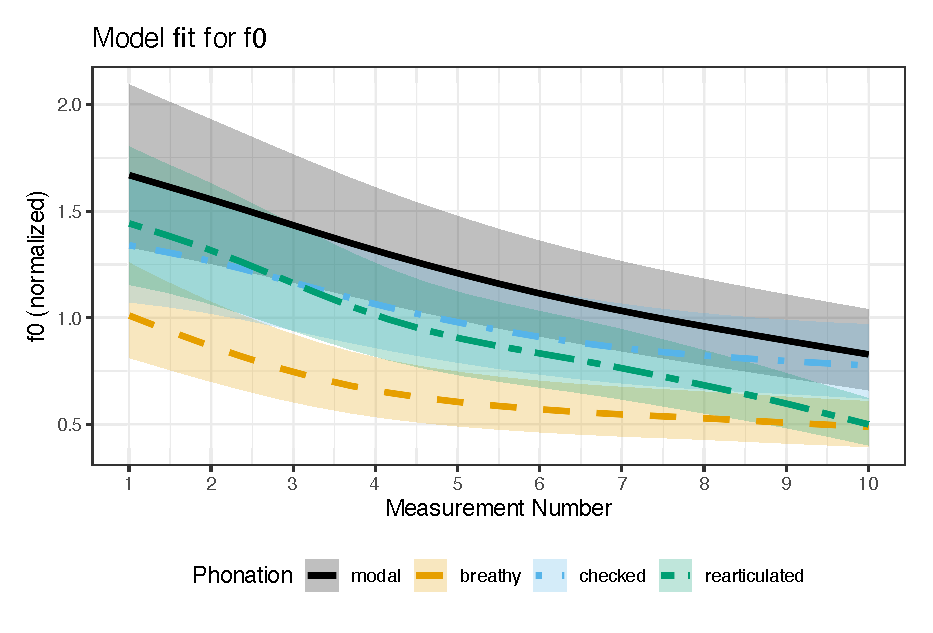
\includegraphics[width = \linewidth]{images/LCH_GAMMs/f0_model_fit.eps}
    \caption{Model fit for \textit{f}0. Each line represents the predicted values from the GAMM for each of the phonations over time. The shaded area represents the 95\% confidence interval.}
    \label{fig:f0_model_fit}
\end{figure}

The observations from the model fit are only part of the story when evaluating GAMMs. The other piece of evidence that we need is whether or not the differences that we observe in the model fit are significant. This is done through difference plots that compare the values for a given comparison (in this case modal versus one of the non-modal phonations) and returns whether or not the difference is significant or not. In these plots, the red line indicates that the difference that we observe between modal and the other phonation types is significant. The blue line indicates that the difference between modal and the non-modal phonation is not significant. This method of evaluation is the most common method for evaluating GAMMs (see \cite{soskuthyEvaluatingGeneralisedAdditive2021} for discussion about evaluating GAMMs). 

Figure~\ref{fig:f0_model_diff} shows the corresponding difference plot for \textit{f}0. The leftmost panel shows the difference plot between modal and breathy voice. The red line indicates that the differences we observed between modal and breathy voice in Figure~\ref{fig:f0_model_fit} is significant across the entire length of the vowel. The center panel shows the differences between modal and checked voice is not significant at any point during the vowel and in terms of \textit{f}0 there is no difference between these two phonations. The rightmost panel shows the difference between modal and rearticulated voice is also not significant for the first part of the vowel. However, beginning at about measurement number 7, we see that the differences are significant.

\begin{figure}[h!]
    \centering
    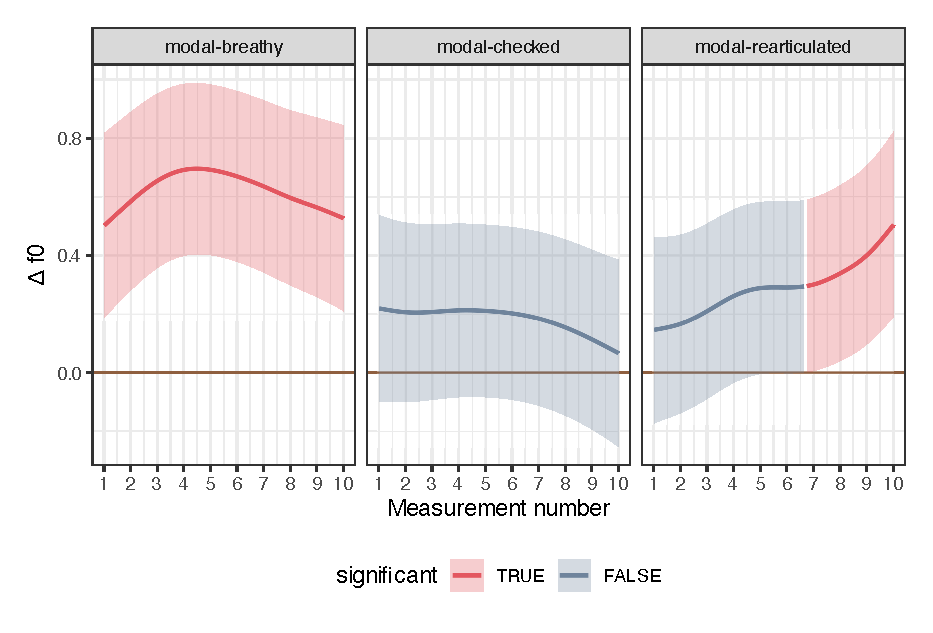
\includegraphics[width = \linewidth]{images/LCH_GAMMs/f0_model_diff.eps}
    \caption{Plot of the difference between modal and each of the non-modal phonation types.}
    \label{fig:f0_model_diff}
\end{figure}

This suggests that in terms of \textit{f}0, breathy voice is significantly different from modal voice throughout the entire duration of the vowel. This is consistent with descriptions for breathy voice cross-linguistically where one of its acoustic cues is a lower \textit{f}0 than modal vowels \citep[e.g.,][]{hillenbrandAcousticCorrelatesBreathy1996}. Whereas rearticulated vowels are only significantly different from modal vowels for the final third of the vowel. The results suggest that in terms of \textit{f}0 perturbation only rearticulated vowels show phasing. 
%--------------------------------------------------------------------------
\subsection{Harmonic-to-noise ratio} \label{sec:model_hnr}
%--------------------------------------------------------------------------

The model fit for HNR < 1500 Hz is shown in Figure~\ref{fig:hnr_model_fit}. In the model fit, we see that modal voice has the highest predicted values for HNR < 1500 Hz, which is consistent with previous research that has shown that modal voice has a higher HNR than non-modal phonation types \citep[e.g.,][]{blankenshipTimeCourseBreathiness1997,blankenshipTimingNonmodalPhonation2002,dekromCepstrumBasedTechniqueDetermining1993,garellekTimingSequencingCoarticulated2012,garellekPhoneticsVoice2019,gerrattTaxonomyNonmodalPhonation2001}. Additionally we see that the three non-modal phonations are all very similar to each other. Checked vowels, however, shows a dipping at the end of the vowel indicating more noise in the signal. 

\begin{figure}[h!]
    \centering
    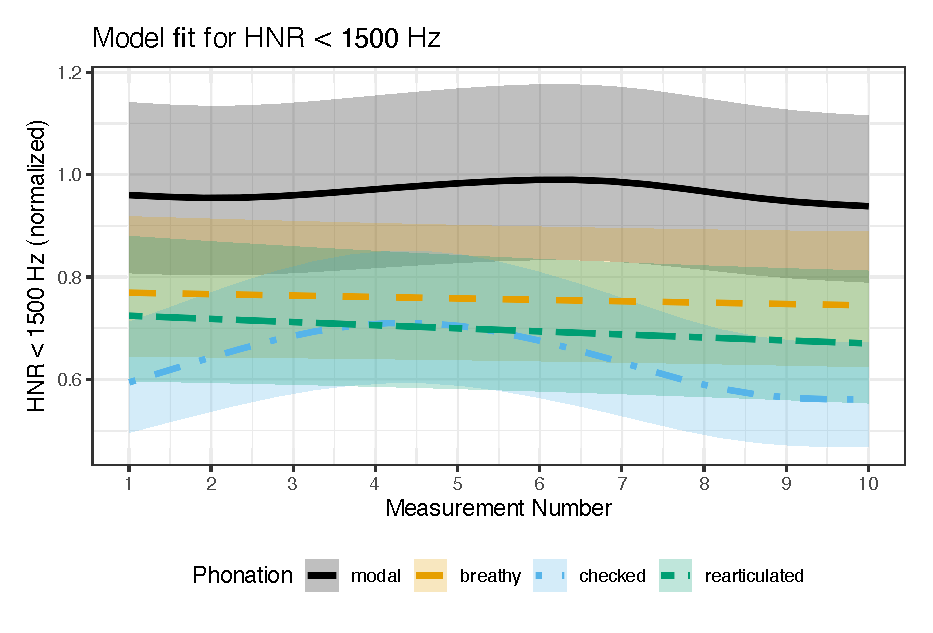
\includegraphics[width = \linewidth]{images/LCH_GAMMs/hnr15_model_fit.eps}
    \caption{Model fit for HNR. Each line represents the predicted values from the GAMM for each of the phonations over time. The shaded area represents the 95\% confidence interval.}
    \label{fig:hnr_model_fit}
\end{figure}  

Figure~\ref{fig:hnr_model_diff} shows the difference plots for each of the non-modal phonations. Similar to Figure~\ref{fig:f0_model_diff}, we see that the leftmost panel shows the difference between modal and breathy voice. This difference is significant from measurement number 4 to halfway between measurements 8 and 9. 

The center and leftmost panels show that the difference between modal and the non-modal phonations is significant across the entire length of the vowel. This indicates that checked and rearticulated vowels are associated with greater aperiodicity across the entire length of the vowel.

\begin{figure}[h!]
    \centering
    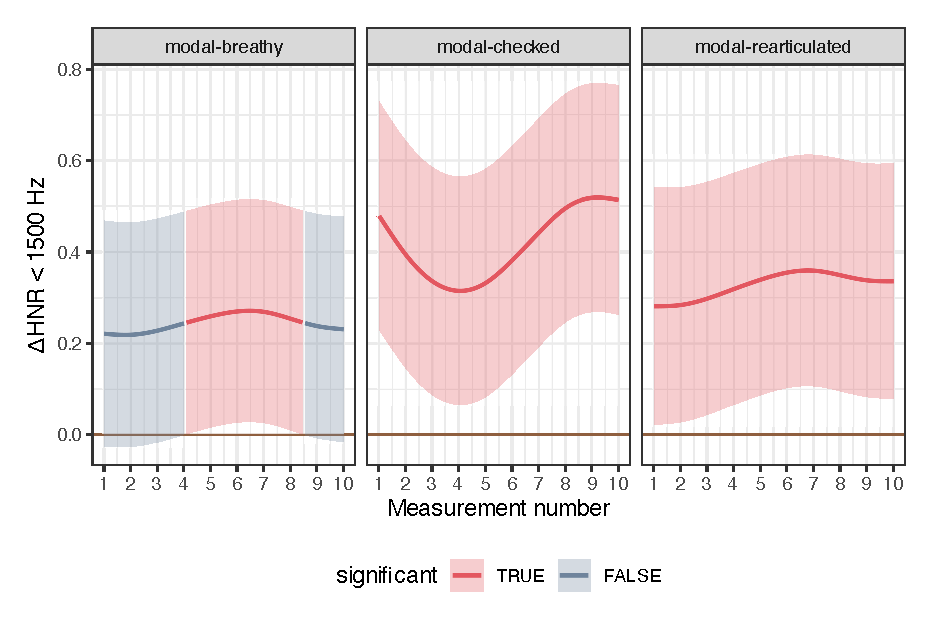
\includegraphics[width = \linewidth]{images/LCH_GAMMs/hnr15_model_diff.eps}
    \caption{Plot of the difference between modal and each of the non-modal phonation types.}
    \label{fig:hnr_model_diff}
\end{figure}

From HNR < 1500 Hz, we see that all three non-modal phonations have more noise in their signal than modal vowels. As I discussed in Section~\ref{sec:bagging_hnr}, HNR measures are typically associated with aperiodicity in the signal. If there is phasing between modal phonation and non-modal phonation as predicted by \citet{silvermanLaryngealComplexityOtomanguean1997}, we would expect to see that these phonations should have a periods where they exhibit more modal-like properties or are not significantly different from modal phonation, which is what we observe with only breathy voice. Breathy vowels show a period of greater aperiodicity than modal vowels in the second half of the vowel, especially if we ignore the interval between 9 and 10 due to coarticulation with the surrounding consonants. Furthermore, this indicates that there is a phasing relationship in breathy vowels where the first half of the vowel is modal and the second half is breathy. 
%--------------------------------------------------------------------------
\subsection{Strength of excitation} \label{sec:model_soe}
%--------------------------------------------------------------------------

As previously discussed in Section~\ref{sec:dt_soe}, SoE is a acoustic measure that correlates to the strength of voicing. Figure~\ref{fig:soe_model_fit} shows the model fit for SoE. In the model fit, we see that modal voice has the highest predicted values for SoE, which is consistent with \citet{garellekVoicingGlottalConsonants2021} where modal vowels are associated with a higher SoE than non-modal phonation because of the greater strength in voicing. 

Breathy voice is identical to modal voice until just after measurement number 2 and then begins to decrease but become identical with modal vowels shortly after measurement number 9. Checked vowels vowels are similar to breathy vowels in that they are identical with modal vowels until just after measurement number 2. However, checked vowels have a sharp decrease in SoE throughout the vowel until measurement number 10. Rearticulated vowels, however, begin lower than the other three phonations but increase in SoE until they are identical with modal voice between measurements 8 and 9. 

\begin{figure}[h!]
    \centering
    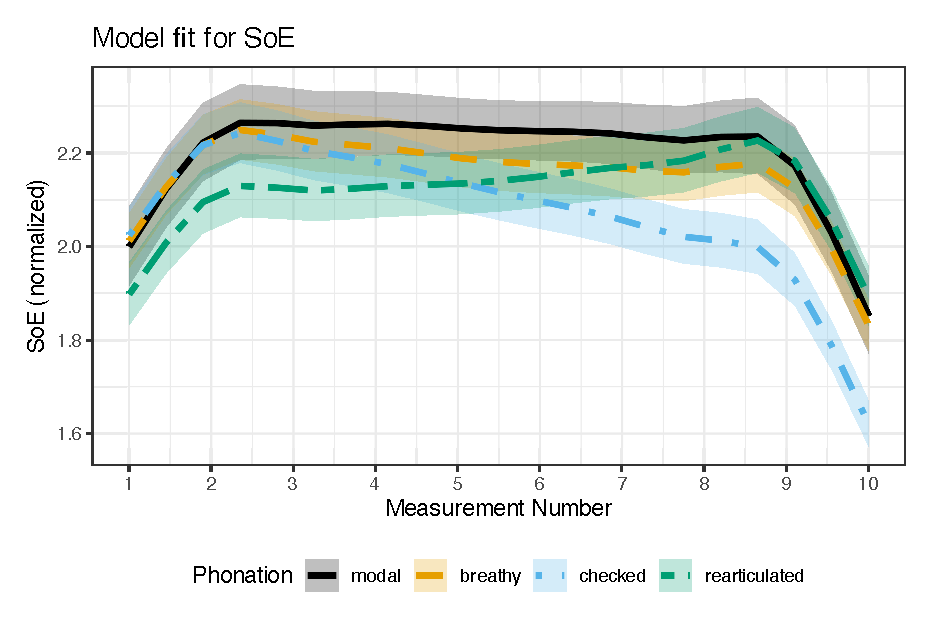
\includegraphics[width = \linewidth]{images/LCH_GAMMs/soe_model_fit.eps}
    \caption{Model fit for SoE. Each line represents the predicted values from the GAMM for each of the phonations over time. The shaded area represents the 95\% confidence interval.}
    \label{fig:soe_model_fit}
\end{figure}

In evaluating whether or not the observed differences from the model fit are significant or not, we can again turn to difference plots to help us determine which differences were significant or not. Figure~\ref{fig:soe_model_diff} shows the difference plots for each of the non-modal phonations. 

The leftmost panel shows the difference between modal and breathy voice. The differences we observed between modal and breathy vowels were only significant between measurement numbers 4 and 8. This is very similar to what we observed in Figure~\ref{fig:hnr_model_diff} for HNR < 1500 Hz. For breathy vowels, we can ignore the interval between measurements 9 and 10 because of the coarticulation with the surrounding consonants.

The center panel shows the difference between modal and checked voice. We observe that checked vowels are significantly different from modal vowels from measurement number 3 to the end of the vowel. However, we can consider the interval between measurements 9 and 10 because checked vowels have a phontactic restriction in the nominal domain that prevents them from occurring in closed syllables. The only time they can accure in a closed syllables is across when a morpheme boundary intervenes like in the word \textit{beku'=nh} [bekuˀ=ŋ] `the dog' where the checked vowel occurs at a morpheme boundary. 

The rightmost panel shows the difference between modal and rearticulated voice. The differences we observed between modal and rearticulated vowels were only significant between measurement numbers 1 and just past 7. 

\begin{figure}[h!]
    \centering
    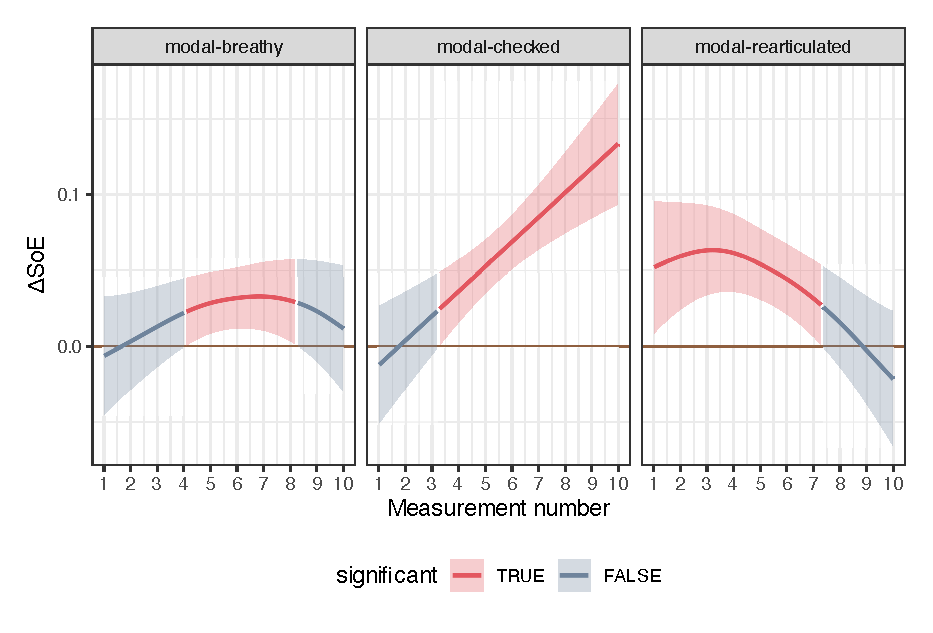
\includegraphics[width = \linewidth]{images/LCH_GAMMs/soe_model_diff.eps}
    \caption{Plot of the difference between modal and each of the non-modal phonation types.}
    \label{fig:soe_model_diff}
\end{figure}

From the SoE measure, we see that the strength of voicing is not drastically different between modal and non-modal phonation. This suggests that the non-modal phonations are not as strongly articulated in SLZ when compared to non-modal phonation in other languages \citep[e.g.,][]{garellekVoicingGlottalConsonants2021,garellekMarginsPhonologyPhonetics2025,wellerInteractionsToneGlottalization2023,wellerLexicalToneVowel2023,wellerVoiceQualityTone2024}. This weak articulation is predicted 

%--------------------------------------------------------------------------
\section{Discussion}\label{sec:discussion_of_lc}
%--------------------------------------------------------------------------

\citet{humbertConsonantTypesVowel1978} 


%--------------------------------------------------------------------------
\section{Conclusion}\label{sec:conclusion_of_lc}
%--------------------------------------------------------------------------
